%!TEX root = ../gronskiy_phd_thesis.tex 
\chapter[Does the Free Energy Define the Model Behavior?]{Does the Free Energy Define \\ the Model Behavior?}
\label{ch:smbp_and_rem}

\hfill
\begin{minipage}[t]{.75\textwidth}
\textit{``When I see a bird that walks like a duck and swims like a duck and
  quacks like a duck, I call that bird a duck.''} \\
  \hrule
  \vspace{.2cm}
  \hfill
  \textsc{---  James Whitcomb RILEY} (attr.)
\end{minipage}

\section{Introduction}

\subsection{Motivation}

Random combinatorial optimization problems exhibit a highly complex structure
with a spin glass behavior~\citep{Mezard87,SK:CG:MV:Science1983}. Optimization
algorithms for these problems are slowed down by fluctuations in the problem
instances when they search for solutions with low costs. Conceptually, we
consider an optimization algorithm as a mapping from an input space of random
instances to an output space of solutions and such algorithms should sample
``typical'' solutions from appropriate posterior distributions. In this chapter,
we concentrate on maximum entropy sampling principles guided by Gibbs
distributions to study information theoretic properties of random combinatorial
optimization problems and their search landscape.  Analytical computation of
free energy, entropy and other macroscopic thermodynamical properties enables us
to understand the solution structure of a large system, but~--- as already
clarified in~Chapter~\ref{ch:free_energy},~--- this goal has been
known to be notoriously difficult and challenging from a mathematical
standpoint~\citep{talagrand03}. 

While we solved this problem for specific cases (Chapter~\ref{ch:free_energy})
with the purpose of applying in to robust optimization (Chapters~\ref{ch:gen_appch}
and~\ref{ch:mst}), here we will be interested in a more general consequence of
such results: a relation between the Random Energy Model (REM;
see~\citealp{derrida81}) and the Sparse Minimum Bisection Problem (sMBP;
see~Section~\ref{sec:free_mbp-problem}).

% Why are we interested in the relations between REM and sMBP? \\

Why are the relations between REM and sMBP of interest?  The REM does not
introduce any statistical dependencies between solutions. Therefore,
optimization algorithms have to exhaustively inspect all exponentially many
solutions of REM to find the one with minimal costs. Sparse Minimum Bisection
introduces correlations between solutions but they are asymptotically so weak
that they do not change the free energy. Since the free energy is the moment
generating function of the Gibbs distribution we hypothesize that the Gibbs
distributions of both problems are equivalent in terms of Kullback-Leibler
divergences. If this claim would hold then we would not be able to efficiently
search for low cost solutions of sMBP.

\subsection{Contributions and Outline of the Chapter}
\label{sec:smbp_and_rem_contribs}

In this chapter, we revisit the idea of characterizing structural
information in solutions for combinatorial problems by 
information theoretic properties. 

More specifically:
%
\begin{itemize}
  \item we revisit results on the asymptotic behavior of the free
    energy~(Chapter~\ref{ch:free_energy}) on obtaining bounds on the free energy of
    solutions for the sMBP with random edge weights;

  \item these results reveal a remarkable phenomenon that the
    free energy of sMBP behaves very similarly to that of REM. Specifically, we
    show that the free energy of sMBP with random edge weights exhibits phase
    transitions equivalent to Derrida's REM;

  \item in order to deeper understand this observation and solution structure for
    dependent and independent solutions, we then make and prove statements about
    various ways sMBP and REM can be quantitatively related to each other: we show
    that the Kullback-Leibler divergence between Gibbs distributions induced by sMBP
    and REM are bounded, but not zero, which allows to make a conjecture about their
    complexity relations.
\end{itemize}

The chapter is organized as follows. As usual, we start with describing some of
related work in Section~\ref{sec:smbp_rem_related_work}. We then present and
discuss our results about the similar behavior of REM and sMBP in
Section~\ref{sec:smbp_rem_similar}. We speculate on the ways to interpret these
results in Sections~\ref{sec:mbp_and_rem_how_similar}
and~\ref{sec:rem_conclusion}.


\section{Background and Related Work Overview}
\label{sec:smbp_rem_related_work}

Information theory, statistical mechanics and combinatorial optimization in
large disordered systems have been disciplines enjoying several waves of
intensive research. The first wave, associated exclusively with the statistical
mechanics, was marked by the works of~\citet{sk75spinb} or~\citet{derrida81} on
mean-field models of spin glasses. For the reasons stated in the introduction,
we concentrate on Derrida's solvable REM. In short, REM is the simplest
example of a disordered system, whose configurations have i.i.d. energies and,
therefore, are not efficiently ``searchable''. It will become important in the
rest of the chapter that REM reflects the situation with no stochastic
dependencies between solutions. This work inspired several continuations, of
which we can mention, e.g., \citep{derrida86} as a generalization of REM,
or~\citep{Aizenman1987} as exact solution of Sherrington-Kirkpatrick
model~\citep{sk75spin}.

\index{Traveling Salesman Problem}
\index{TSP|see{Traveling Salesman Problem}} 
The second wave of interest was associated not exclusively with statistical
mechanics, but also researched its connection to combinatorial optimization.
Inspired by the work of Derrida, \citet{mezard84tsp} considered the Traveling
Salesman Problem (TSP) as a large disordered system which seeks to optimize its
energy defined by respective \textit{Hamiltonians}\index{Hamiltonian} (see
Section~\ref{sec:background_disordered_systems}). This approach to view a
combinatorial optimization problem from the statistical mechanics prospective
turned out to be extremely fruitful: we recommend the book~\citep{LUCZAK1994} as
a good overview of the results. We should also mention here the
work~\citep{Auffinger2014} who studied algorithmic complexity from the
statistical mechanics viewpoint.
\index{Complexity}
\index{Algorithmic complexity}

Finally, in the last two decades, many attempts have been made to systematize
approaches traditionally used in statistical mechanics and render them rigorous
in a mathematical sense. Here, we point out the work by
\citet{Bovier2002FreeEnergyFluct}, as well as extensive
reviews by \citet{talagrand03,bovier2012statistical}.

\section{Comparison of REM and sMBP}

\subsection{Random Energy Model (REM)}

\index{Random Energy Model}
\index{REM|see{Random Energy Model}}

The REM introduced by~\citet{derrida81} is a model $\mathcal{P}^\mathrm{rem} =
(\mathcal{X}, \C^\mathrm{rem}, R^\mathrm{rem})$ 
\nomenclature[F, 50]{$(\mathcal{X}, \C^\mathrm{rem}, R^\mathrm{rem})$}{definition of REM\nomnorefeq}%
where the following conditions apply:
\begin{enumerate}
  \item Number of solutions (in the original terminology,
    \textit{configurations}) equals 
    \begin{equation}
      |\C^\mathrm{rem}| = 2^K.
    \end{equation}
  \item Here, the data source $X \in \mathcal{X}$ is a vector of $2^K$ Gaussian
    random variables (for the notation, see
    Definition~\ref{def:optimization_problem_definition}), and all solutions
    $c_i
    \in \C^\mathrm{rem}$ carry costs (in the original terminology,
    \textit{Hamiltonians} or \textit{energy levels})
    \begin{equation}
      R^\mathrm{rem}(c_i, X) = X_i, \;\; \text{where} \;\; X_i \sim \mathcal{N}(0, \sigma^2)
    \end{equation}
    \item The costs $X_i$ are i.i.d.
\end{enumerate}

As Derrida noted in his paper, ``the third property is specific to this model.
It simplifies the model enough to allow us to solve it exactly''. While it is
true for REM, such independence is not characteristic for the most of the
models. The next section which discusses dependencies in sMBP.

\subsection{Similar Behavior of REM and sMBP}
\label{sec:smbp_rem_similar}
Earlier, we introduced the sparsity constraint on $d$ in
Theorem~\ref{thm:sparse_mbp_tight_bound} because without it, the stochastic
dependency between two random solutions for original MBP~\citep{garey79} is very
high. Indeed, in original MBP, any two bisections \textit{always} share edges.
By introducing $d$ we: a) substantially reduce such dependency, but on the other
hand b) do not eliminate it at all, like in REM~\citep{derrida81}. 

But by introducing sparsity, didn't we essentially \textit{transform} MBP into
REM? E.g. one can observe that for classical dependency-free REM, the free
energy asymptotics looks just the same, in particular exhibits the same phase
transition and same phase shapes:

\begin{theorem}[adapted formulation from~\citep{talagrand03}] \label{thm:rem}
  Assume $m = 2^K$ is the number of configurations for the REM model with
  Gaussian cost values, with parameters $\mathcal{N}(0, \tau^2)$. Then the
  free energy rate is (asymptotically in $n \to \infty$) equal to
    \begin{equation} \label{eq:talagrand_rem_with_tau}
      \lim_{n \to \infty} \frac{\E[\log Z]}{\log m}=
      \left\{ \begin{array}{ll}
      \frac{\beta^2 \tau^2}{2 \log m} + 1 & 
      \beta < \sqrt{2 \log m}/\tau,\\
      \frac{\beta \tau \sqrt{2}}{\sqrt{\log m}} & \beta \ge \sqrt{2 \log m}/\tau.
      \end{array}
      \right.
    \end{equation}
\end{theorem}
We note that Talagrand formulated it in a more general setting~\citep[cf.][Prop.
1.1.3]{talagrand03}, which is adapted here for clarity. Choosing $\tau = \sigma
\sqrt{N}$ and applying $\beta$ rescaling from~\ref{def:cts}, we arrive at an
equivalent formulation: for Gaussian cost values with parameters $(0, \sigma^2
N)$, we derive
\begin{equation} \label{eq:talagrand_rem_adapted}
  \lim_{n \to \infty} \frac{\E[\log Z]}{\log m}=
  \left\{ 
    \begin{array}{ll}
      1+\frac{\hat \beta^2\sigma^2}{2}, &
        \hat \beta< \frac{\sqrt{2}}{\sigma},\\
      \hat \beta \sigma \sqrt{2}, & 
        \hat \beta \ge \frac{\sqrt{2}}{\sigma}
    \end{array}
  \right.
\end{equation}
\myremark For non-centered cost values, the necessary
correction similar to the one of~\eqref{eq:sparse_mbp_tight_bound} should be
made on the left-hand side which is trivial.

We are now going to sketch an answer to the following question: how much does
sMBP look like REM? We give the following result and then discuss it. First,
let's make some definitions.

\begin{definition}
  For an sMBP setting stated in Theorem~\ref{thm:sparse_mbp_tight_bound},
  we will call equivalent such a REM, for which the number
  of configurations is equal to $m$ and the cost values are Gaussian with
  parameters $(\mu N,
  \sigma^2 N)$.
\end{definition}
For convenience of the following explanation, let us denote the random source
behind such a REM as $Y$ (analogically to $X$ in case of sMBP). Hence for REM,
the cost values $R(c, Y) \sim \mathcal{N}(\mu N, \sigma^2 N)$ and all are
independent. We denote the respective Gibbs distributions $\psmbp_\beta(c | X)$ and
$\prem_\beta(c | Y)$.
\index{Kullback-Leibler divergence}
\begin{theorem}\label{thm:kl_divergence}
  The rate of the KL-divergence between configurations' Gibbs distributions for sMBP 
  and equivalent REM is non-zero and exhibits a phase transition.
  \begin{equation}
    \frac{\Expct_{X, Y}[\KL(\prem_\beta \| \psmbp_\beta)]}{\log m} = 
      \left\{ 
        \begin{array}{ll}
          \hat\beta^2 \sigma^2 &
            \hat \beta< \frac{\sqrt{2}}{\sigma},\\
          \hat \beta \sigma \sqrt{2}, & 
            \hat \beta \ge \frac{\sqrt{2}}{\sigma}
        \end{array}
      \right.
  \end{equation}
  \nomenclature[F, 50a]{$\prem_\beta(c "| X)$}{Gibbs distribution of REM model}%
  \nomenclature[F, 50c]{$\psmbp_\beta(c "| X)$}{Gibbs distribution of sMBP}%
\end{theorem}

\paragraph{Proof}
In the first part of the proof, we will omit the expectation for the sake of
brevity.
%
\begin{align}
\MoveEqLeft \KL(\prem_\beta \| \psmbp_\beta) = \sum_c \prem_\beta(c\vert Y) \log
  \frac{\prem_\beta(c\vert Y)}{\psmbp_\beta(c\vert X)} = \notag \\
  &= \sum_c \prem_\beta(c\vert Y) 
    \left(  
      \log \frac{e^{-\beta \Rrem(c,Y)}}{\Zrem(Y)} \right. \notag \\
      &\qquad\qquad\qquad\qquad
      \left. - \log \frac{e^{-\beta \Rsmbp(c,X)}}{\Zsmbp(X)}
    \right) \notag \\
  &=  \sum_c \prem_\beta(c\vert Y) 
    \left(  \vphantom{\sum}
      \log e^{-\beta \Rrem(c,Y)}   \right. \notag \\
      &\qquad\qquad\qquad - \log e^{-\beta \Rsmbp(c,X)} \notag \\
      &\qquad\qquad\qquad \left. - \log \Zrem(Y) + \log \Zsmbp(X)
      \vphantom{\sum}\right) \notag \\
  &= -\beta \sum_c \prem_\beta(c\vert Y) 
    \Bigl( \Rrem(c,Y) - \Rsmbp(c,X) \Bigr) \notag \\
      &\qquad\qquad\qquad  - \log \Zrem(Y) + \log \Zsmbp(X) 
\end{align}
Returning to the expectation $\Expct_{X,Y}$ and recalling that all the
sMBP-related terms depend on $X$ and all the REM-related terms depend on $Y$, we can continue:
\begin{align}
  \MoveEqLeft -\beta \Expct_{X,Y} \biggl[\sum_c \prem_\beta(c\vert Y) 
    \Bigl( \Rrem(c,Y) - \Rsmbp(c,X) \Bigr) \biggr] \notag \\
      &\qquad\qquad  
        \underbrace{
            {} - \Expct_Y [\log \Zrem(Y) ]
            + \Expct_X [\log \Zsmbp(X)]
          }_{
          \text{
            cancel out due to Thm.~\ref{thm:sparse_mbp_tight_bound} and \ref{thm:rem}}
          } \notag \\
  &= -\beta  
    \Bigl( \Expct_{Y} \Bigl[\sum_c \prem_\beta(c\vert Y) \Rrem(c,Y) \Bigr] \notag \\
        &\qquad\qquad - \Expct_Y 
          \underbrace{\sum_c \prem_\beta(c\vert Y)}_{1} \cdot 
          \underbrace{\vphantom{\sum_c}\Expct_X \Rsmbp(c,X)}_{\mu N} \Bigr) \notag \\
  &= \beta \mu N + \beta \Expct_Y \Bigl[\frac{d}{d\beta} \log \Zrem(Y)\Bigr].
\end{align}
By the argument of dominated convergence theorem, we can under mild conditions
interchange expectation and differentiation, which together
with~\eqref{eq:talagrand_rem_with_tau} and~\eqref{eq:talagrand_rem_adapted}
leads to
\begin{equation}
  \Expct_{X, Y}[\KL(\prem_\beta \| \psmbp_\beta)] = 
    \left\{ 
      \begin{array}{ll}
        \hat\beta^2 \sigma^2 \log m &
          \hat \beta< \frac{\sqrt{2}}{\sigma},\\
        \hat \beta \sigma \log m \sqrt{2}, & 
          \hat \beta \ge \frac{\sqrt{2}}{\sigma},
      \end{array}
    \right.
\end{equation}
which completes the proof of theorem.
\QEDA

\subsection{Consequences of Similar Behavior of REM and sMBP}

We now discuss this result. There are several observations to be made about the
whole line of research reflected in
Theorems~\ref{thm:sparse_mbp_tight_bound},~\ref{thm:rem}
and~\ref{thm:kl_divergence}.

\begin{figure}[th!]
  \centering
  \begin{subfigure}[b]{.48\textwidth}
      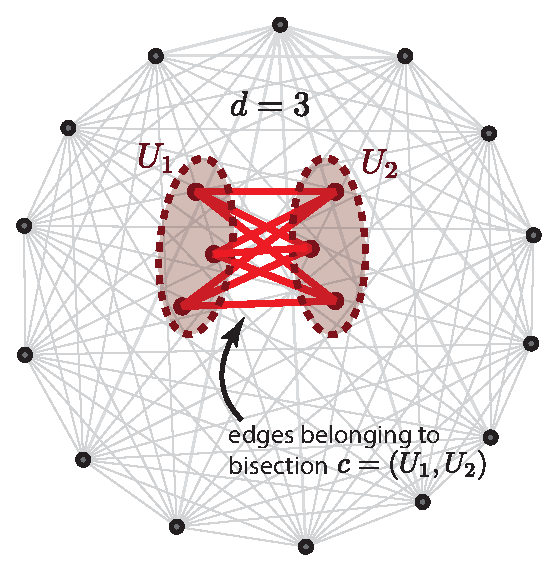
\includegraphics[width=\linewidth]{figures/ch_smbp_and_rem/different_solution_overlaps}
      \caption{Solution to an sMBP problem}
      \label{fig:ch_rem_smbp_illustration-0}
  \end{subfigure}
  \hfill
  \begin{subfigure}[b]{.48\textwidth}
      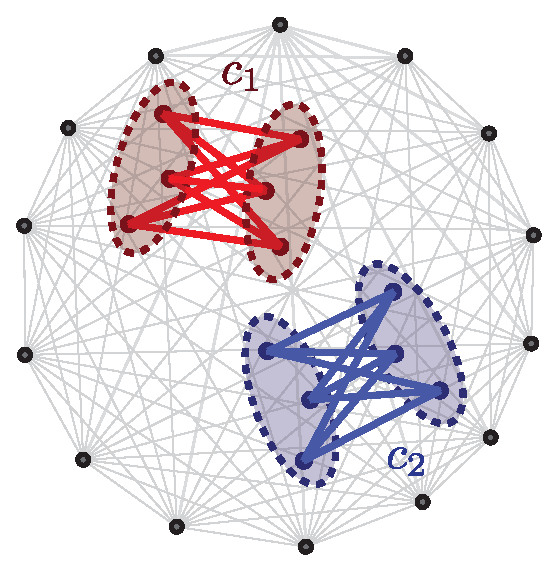
\includegraphics[width=\linewidth]{figures/ch_smbp_and_rem/different_solution_overlaps_1}
      \caption{No overlap at all}
      \label{fig:ch_rem_smbp_illustration-1}
  \end{subfigure}
  \\[.5cm]
  \begin{subfigure}[b]{.48\textwidth}
      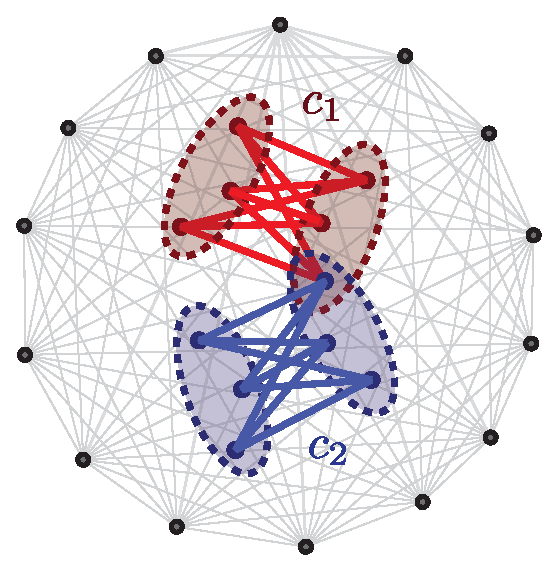
\includegraphics[width=\linewidth]{figures/ch_smbp_and_rem/different_solution_overlaps_2}
      \caption{Vertex overlap, but no edge overlap}
      \label{fig:ch_rem_smbp_illustration-2}
  \end{subfigure}
  \hfill
  \begin{subfigure}[b]{.48\textwidth}
      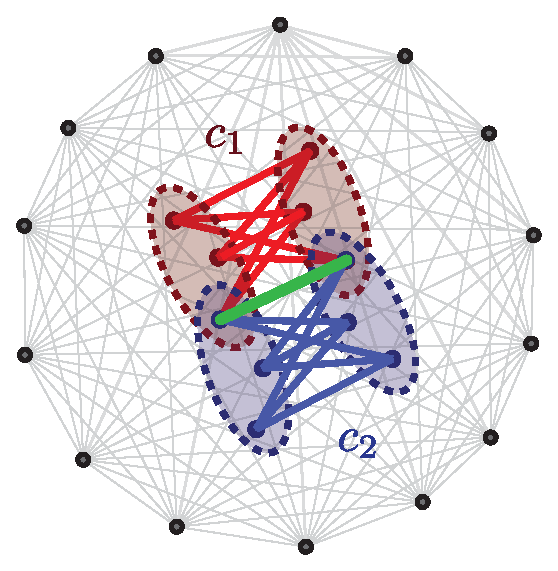
\includegraphics[width=\linewidth]{figures/ch_smbp_and_rem/different_solution_overlaps_3}
      \caption{Only edge overlap counts}
      \label{fig:ch_rem_smbp_illustration-3}
  \end{subfigure}
  \\[.5cm]
  \caption{Illustration of various types of overlaps. Only case \textbf{(d)}
  contributes to statistical dependence between costs of solutions. Carefully
  computing edge overlap can make a huge step forward in understanding higher
  moments of $\log Z$ (in Lemma~\ref{lem:expct_d_asymptotics} we computed only
  expected value).}
  \label{fig:ch_rem_smbp_illustration}
\end{figure}

First, Theorems~\ref{thm:sparse_mbp_tight_bound},~\ref{thm:rem}
and~\ref{thm:kl_divergence} can be interpreted as follows: they yield the
similarity of both problems in terms of macroscopic thermodynamical properties
like free energy rate, but at the same time they convey their difference in
terms of KL-divergence rate: by definition of $\KL$, it measures the amount of
information one might gain (or lose) by assuming $\prem$ instead of $\psmbp$ or
vice versa. The fact that the expected KL-divergence rate is non-zero allows us
to say that sMBP and REM are still different in terms of their distributions.

Second, and probably most importantly, due to the same line of reasoning as in
Theorem~\ref{thm:kl_divergence}, we can conclude that a KL-divergence between
every pair $({\prem}', {\prem}'')$ of independent (that is, with independent
$Y'$ and $Y''$) equivalent REMs is identical to that of $(\prem, \psmbp)$. This
highlights the fact that for full understanding of relations (similarities and
differences) between them one needs to properly quantify this difference in
terms of higher moments and not only \textit{expectation} of KL-divergence rate.

It is important to realize that the higher moments of the KL-divergence can be
most likely controlled by the higher moments of $\log Z$, i.e. $\Var[\log Z]$
and so on. 

The necessary understanding of the behavior of $\Var[\log Z]$, in turn, can be
reached via careful computing of higher moments of edge overlap $D$ of the two
solutions $c_1$ and $c_2$ (illustrated in
Figure~\ref{fig:ch_rem_smbp_illustration}): one can see this, for example,
from the proof of Theorem~\ref{thm:sparse_mbp_tight_bound}, where we have 
\begin{equation*}
  \Var Z \sim (\Expct Z)^2 \bigl( \sigma^2 \beta^2 \Expct_\D D \bigr)
\end{equation*}
as an intermediate result. There exists evidence of a possibility to use 
Taylor expansions to express higher moments of $\log Z$ via those of $Z$.

\section{Comparison of REM and non-sparse MBP}
\label{sec:mbp_and_rem_how_similar}

Interesting question arises: can we say anything about non-sparse (i.e. case
when $d \not \ll n$) MBP? Note that in Section~\ref{sec:free_energy_in_general_case}
of Chapter~\ref{ch:free_energy} we made a conjecture which is backed up by
extensive simulations, which we restate here:

\newtheorem*{adhocconj}{Conjecture~\ref{ad-hoc}}
\begin{adhocconj}[see Section~\ref{sec:free_energy_in_general_case}]
Consider a class of combinatorial optimization problems complying with Common
Theorem Setting, weights $W_i$ having mean $\mu$ and variance $\sigma^2$. Then
the free energy satisfies
\begin{equation*}
    \lim_{n\to \infty} \frac{\E[\log Z(\beta, X)] +\hat \beta \mu \sqrt{N\log m}}{\log m}
    =
    \begin{cases}
        1 + \alpha^2\frac{\hat{\beta}^2\sigma^2}{2},
            &\hat{\beta} < \frac{\sqrt{2}}{\alpha\sigma} \\
\alpha\hat{\beta}\sigma\sqrt{2}, &\hat{\beta} \geq \frac{\sqrt{2}}
{\alpha\sigma}
    \end{cases}
\end{equation*}
for some $\alpha \ge 1$,
where $\alpha$ is well approximated by
\begin{equation*}
    \alpha 
      = \sqrt{\frac{\E_X\Var_{\mathcal{D}} R(c,X)}{\E_{\mathcal{D}}\Var_X R(c,X)}} 
      = \sqrt{\frac{\E_X\Var_{\mathcal{D}} R(c,X)}{N\sigma^2}}
\end{equation*}
\end{adhocconj}

It is instructive to note here that, loosely speaking, parameter $\alpha$
represents the ratio variability across solutions (nominator) and the
variability inside each solution (denominator). The higher the dependence is, the 
less variability across solutions exists. 

Apparently $\alpha = 1$ corresponds to a case of no dependencies (sMBP), while
lower alpha corresponds to higher levels of dependencies. And again, to further
back up this conjecture, one has to develop the understanding of
$\Var_{\mathcal{D}} R(c, X)$, i.e. variance of costs for uniformly chosen
solutions, which boils down to taking overlaps under control (computing
$\Var_\mathcal{D} [D]$ analogically to $\Expct_\mathcal{D}[D]$ as we did in
Lemma~\ref{lem:expct_d_asymptotics}.

\section{Discussion and Conclusion}
\label{sec:rem_conclusion}

The geometry of random combinatorial optimization problems is often
characterized by exponentially many local minima which prevent an
efficient search for low cost solutions. In this chapter, we have
studied random instances of sparse Minimum Bisection Problem which
exhibit a statistical behavior very similar to that of the Random Energy
Model. This similarity between the Gibbs distributions for REM
instances and for sMBP instances is documented by identical values for
the free energies and for the Kullback-Leibler divergences between
pairs of distributions. 

Furthermore, this equivalence also suggests that the computational complexity of
REM and sMBP might be the same and, consequently, random instances of sMBP might
not be efficiently optimized due to the lack of search information as in REM. As
a future research direction we plan to analyze the finite $\log m$ corrections
to estimate the convergence rate of the free energy toward its asymptotic limit.
Another open question remains if there exist REM instances that are arbitrarily
close (w.r.t. KL-divergence) to sMBP instances in the asymptotic limit,
explaining why we cannot find efficient optimization schemes for sparse Minimum
Bisection.

For answering the last question, we have highlighted the importance of developing a better
understanding of the higher moments of the solutions overlap
(Figure~\ref{fig:ch_rem_smbp_illustration}), since the proofs we gave earlier
yield that controlling the dependency between the solutions gives us the essential 
information about the problem's (dis)similarity from REM, where such dependencies
don't exist at all.
